% LaTeX path to the root directory of the current project
\providecommand{\econtexRoot}{}
\renewcommand{\econtexRoot}{.}
\documentclass[../CGMPort.tex]{subfiles}
\onlyinsubfile{% https://tex.stackexchange.com/questions/463699/proper-reference-numbers-with-subfiles
    \csname @ifpackageloaded\endcsname{xr-hyper}{%
      \externaldocument{\econtexRoot/BufferStockTheory}% xr-hyper in use; optional argument for url of main.pdf for hyperlinks
    }{%
      \externaldocument{main}% xr in use
    }%
    \renewcommand\labelprefix{}%
    % Initialize the counters via the labels belonging to the main document:
    \setcounter{equation}{\numexpr\getrefnumber{\labelprefix eq:AAgg}\relax}% eq:AAgg is the last numbered equation in the main text; start counting up from there
}

\begin{document}

\section{Comparison with CGM}\label{sec:Comparison}

In this section, we compare the policy functions that we obtain using HARK, with those that are obtained using CGM's publicly available 
\href{http://faculty.london.edu/fgomes/cgmcode.ZIP}{\texttt{Fortran 90 code}}.

We attempted to execute the authors' code as-is, but obtained a ``division by zero'' error, apparently caused by one of the asset grids starting at $0$,
allowing the possibility of a $0$-level of consumption to be evaluated in the
utility function. We fixed the issue by making said grid start at $1$. The
figures produced in this section use the policy functions outputted by the
author's code after this fix. 

Figures \ref{fig:heatmapCons} and \ref{fig:heatmapRshare} display policy 
functions for consumption and risky portfolio shares obtained with CGM's code and our HARK implementation, and their substantial differences.

\begin{figure}[h]
	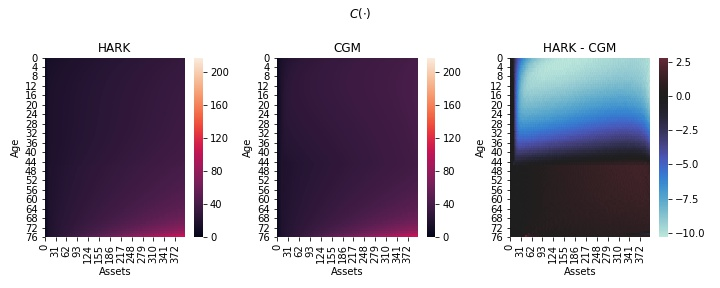
\includegraphics[width = \linewidth]{\FigDirPython/Cons_Pol_Compare}
	\caption{Consumption policy functions in HARK and CGM's Fortran 
	code.}\label{fig:heatmapCons}
\end{figure}

\begin{figure}[h]
	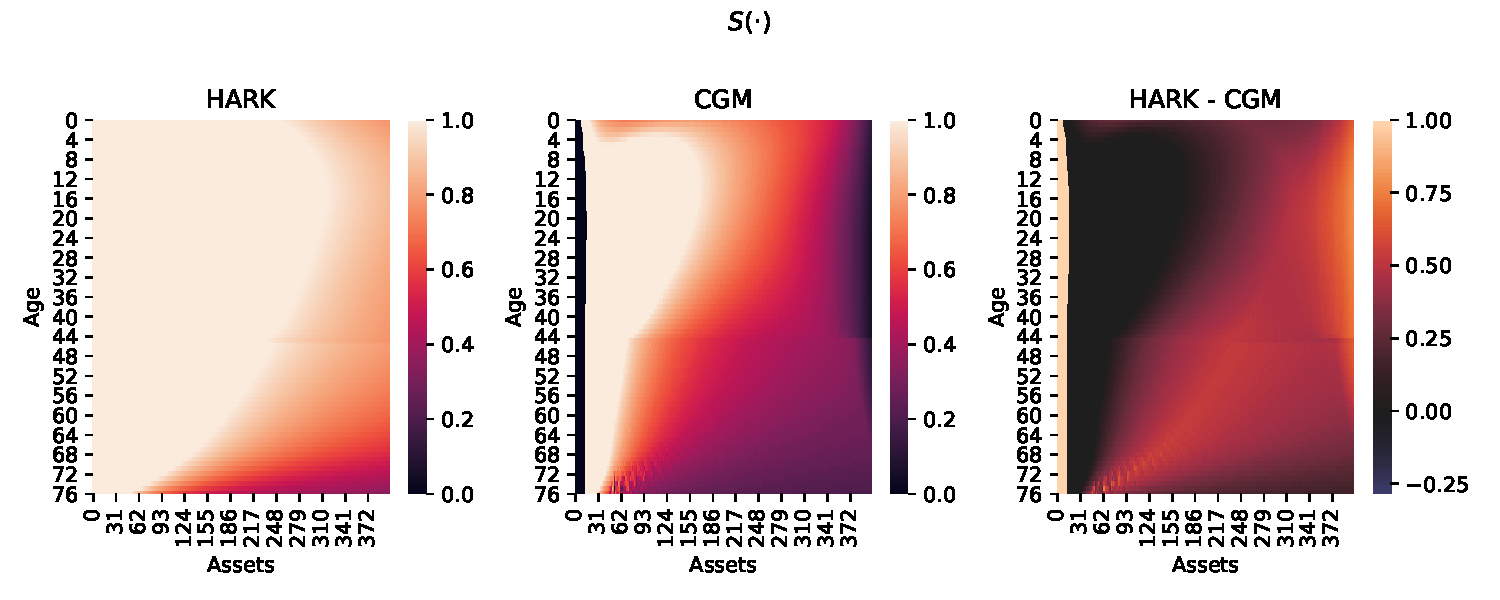
\includegraphics[width = \linewidth]{\FigDirPython/RShare_Pol_Compare}
	\caption{Risky share policy functions in HARK and CGM's Fortran code.}
	\label{fig:heatmapRshare}
\end{figure}

Given the differences, we inspect the second and third-to-last life periods more closely. Figure \ref{fig:pol_funcs_last} presents policy functions and their differences for these periods. The discrepancies are evident.

\begin{figure}[h]
	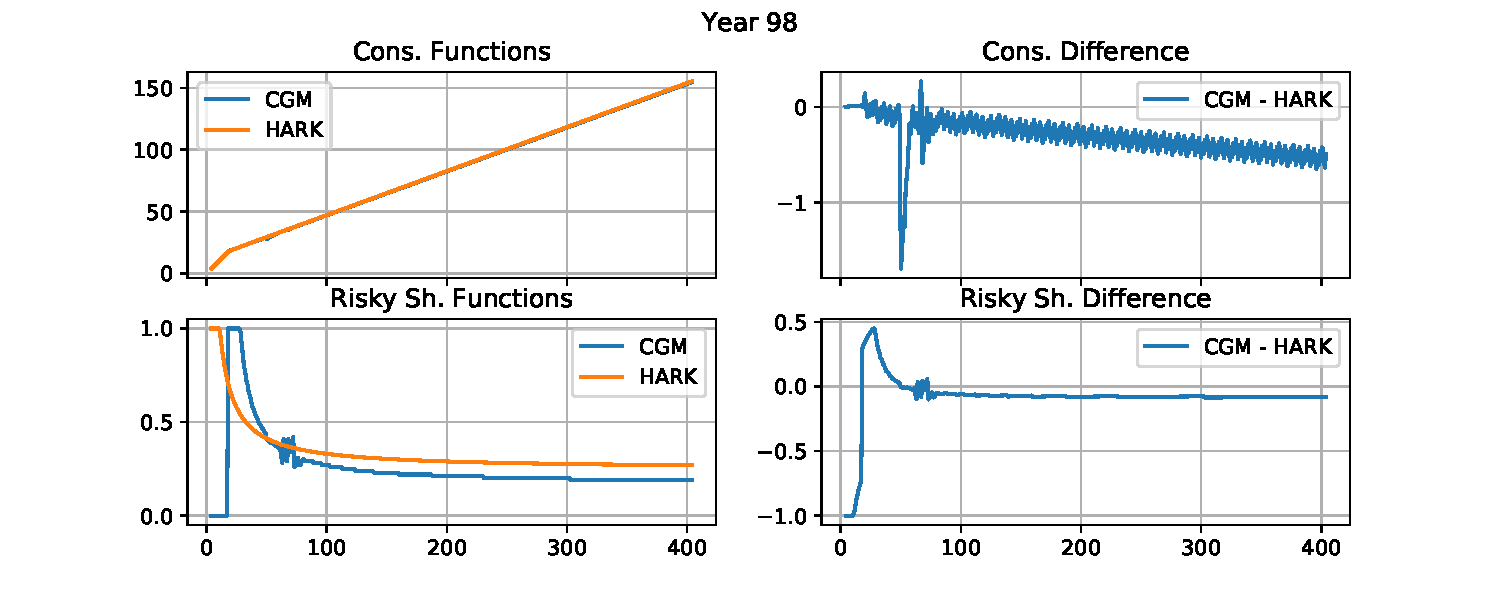
\includegraphics[width = \linewidth]{\FigDirPython/PolFunc_Compare_Y98}
	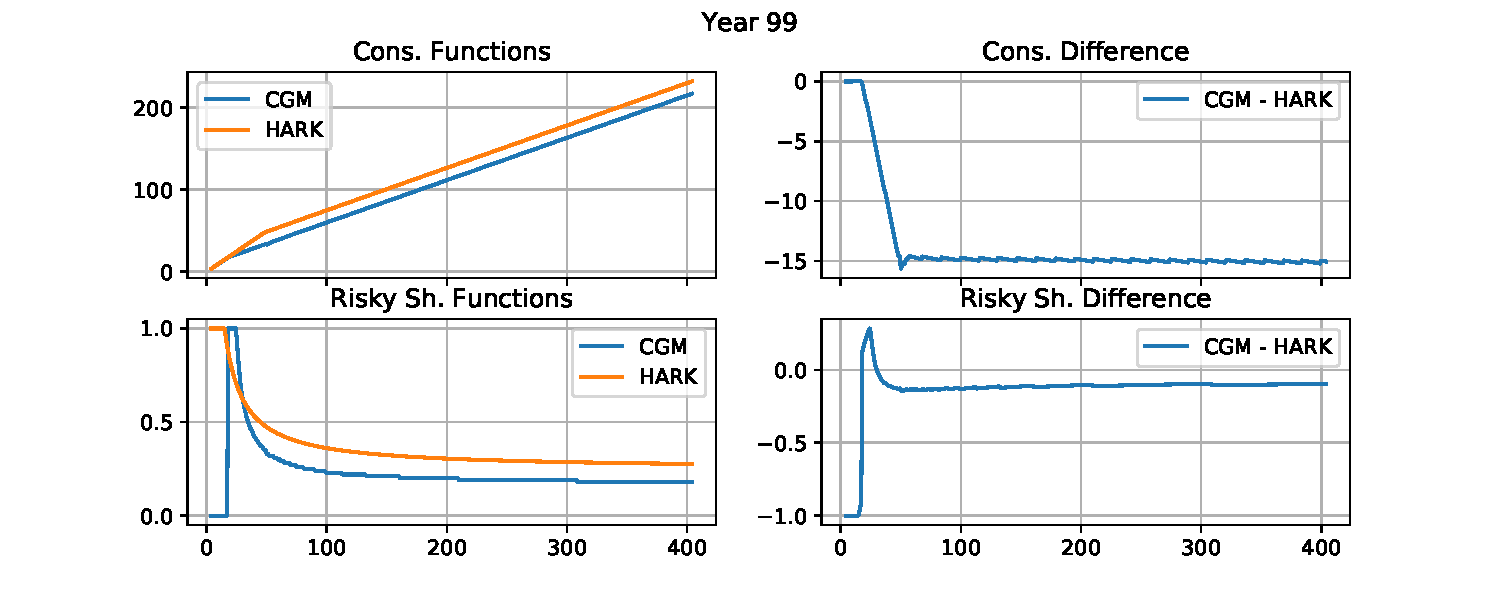
\includegraphics[width = \linewidth]{\FigDirPython/PolFunc_Compare_Y99}
	\caption{Policy functions in the second and third to last periods of life.}
	\label{fig:pol_funcs_last}
\end{figure}


\section{Robustness analyses}\label{sec:Sensitivity}

Given that our main set of results do not align with those of CGM,
we provide a few tests that compare the behavior of the tools that we are using with well known theoretical results.

\subsection{Merton Samuelson's limiting risky share}

Merton and Samuelson (TODO: CITE) show that a consumer with constant relative
risk aversion $\rho$, a risky asset with log-normally distributed returns
with a risk premium $\phi$ and log-standard-deviation $\sigma_r$, and no labor income uncertainty will invest the following share of their income:\footnote{See 
\href{http://www.econ2.jhu.edu/people/ccarroll/public/lecturenotes/AssetPricing/Portfolio-CRRA/}{\texttt{Portfolio-CRRA}}.}
\begin{equation}
	s = \frac{\phi}{\rho \sigma^2_r}.
\end{equation}
This result holds as long as labor income is an \emph{unimportant} source of
wealth for the agent.

To test HARK's implementation, we modify returns to the risky asset to be 
log-normal and keep the rest of the calibration the same. Since labor income
is unimportant for infinitely wealthy agents, our risky portfolio share policy rules must converge to Merton and Samuelson's limit as market resources approach infinity. Figure \ref{fig:MS_share_limit} shows that this is indeed the case.

\begin{figure}[h]
	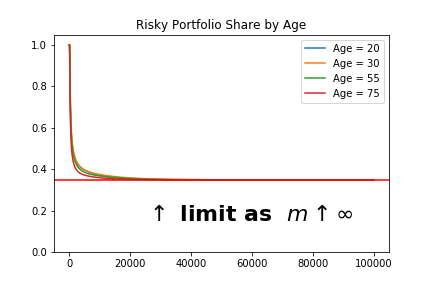
\includegraphics[]{\FigDirPython/Merton_Samuelson_Limit}
	\caption{Merton Samuelson as the limit of the risky asset's portfolio 
		share.}\label{fig:MS_share_limit}
\end{figure}

\subsection{Marginal Propensity to Consume}

\href{http://www.econ2.jhu.edu/people/ccarroll/public/LectureNotes/Consumption/CRRA-RateRisk/}{CRRA-RateRisk}
shows that an infinitely lived agent with no labor income and who can only 
store his wealth in a risky asset with log-normally distributed
returns must have a marginal propensity to consume given by:
\begin{equation}\label{eq:mpc_limit}
	\kappa = 1 - \left( \beta \mathbb{E}_t \left[ \mathfrak{R}^{1-\rho} \right] 
	\right)	^{1/\rho}
\end{equation}
where $\mathfrak{R}$ is the risky asset's return factor.

We modify our calibration to have log-normal returns and to ensure that 
Equation \ref{eq:mpc_limit} is a positive number. We also set the risk free
rate low enough that the agent will allocate all of his wealth to the risky
asset. Since the result holds for infinitely lived consumers with no labor 
income, we should see that our estimated marginal propensity to consume 
converges to $\kappa$ for young and wealthy consumers. Figure \ref{fig:mpc_lim} 
shows that this is indeed the case.

\begin{figure}[h]
	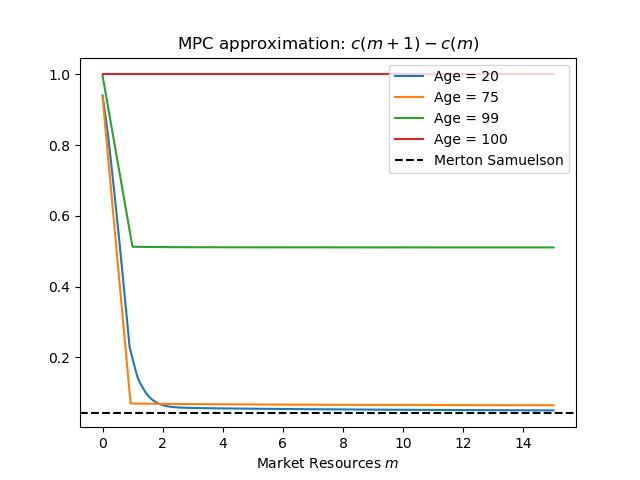
\includegraphics[]{\FigDirPython/MPC_Limit}
	\caption{Marginal propensity to consume as $m \rightarrow \infty$.}
	\label{fig:mpc_lim}
\end{figure}

\subsection{Perfect Foresight analytical solution}

To further verify that HARK's solution algorithm is producing accurate results,
we compare the consumption policy function obtained by the
\texttt{PortfolioConsumerType} class through backward induction with the
analytical expression that can be obtained for consumption in a perfect
foresight setting.

\href{http://www.econ2.jhu.edu/people/ccarroll/public/LectureNotes/Consumption/PerfForesightCRRA/}{PrefForesightCRRA}
shows that a consumer facing no uncertainty will attempt to consume:
\begin{equation}
	c^*_t = \frac{1 - \left[ R^{-1} \left( R \beta \right)^{1/\rho}\right]}{1 - 
	\left[ R^{-1} \left( R \beta \right)^{1/\rho}\right]^{T-t+1}}\times o_t
\end{equation}
where $o_t$ is his overall (human plus non-human) wealth. In the presence of a liquidity constraint, the agent will then consume:
\begin{equation}
	c_t = \min \{ m_t , c^*_t\}
\end{equation}
where $m_t$ are his market resources at time $t$. We refer to this as the 
\emph{true} solution.

We shut down all sources of uncertainty in our calibration and, for ease of
analytical expressions, assume a constant level of income. We then solve the
agent's problem using \texttt{PortfolioConsumerType}'s backward induction
algorithm and compare its solution both with the true solution and the one
obtained by \texttt{PerfForesightConsumerType}, another HARK class representing perfect-foresight consumers.

Figure \ref{fig:pf_compare_lvl} plots consumption functions obtained through the three different methods and three different periods of the agent's life. The \texttt{PortfolioConsumerType} policy function aligns with the true solution, but that of \texttt{PerfForesightConsumerType} does not.

\begin{figure}[h]
	\includegraphics[]{\FigDirPython/Pf_Compare_Lvl}
	\caption{Perfect foresight solutions using different HARK tools.}
	\label{fig:pf_compare_lvl}
\end{figure}

Figure \ref{fig:pf_compare_diff} more closely examines deviations in HARK's
solutions from the true solution. \texttt{PortfolioConsumerType}'s solution
is very close to the true solution at every age and level of wealth with
deviations appearing only around the consumption function's kink, which is
caused by the liquidity constraint that we impose. On the other hand,
the solution provided by \texttt{PerfForesightConsumerType} has substantial
differences in the level of consumption, which widen with the agent's age.

\begin{figure}[h]
	\includegraphics[]{\FigDirPython/Pf_Compare_Diff}
	\caption{Differences from the true perfect foresight solution.}
	\label{fig:pf_compare_diff}
\end{figure}

\end{document}
